%==========================================
% SIBGRAPI 2026 — main track draft
% Cross-domain nuclei segmentation benchmark
%==========================================

\documentclass[10pt,conference]{IEEEtran}

\usepackage{cite}
\usepackage{amsmath,amssymb}
\usepackage{amsthm}
\newtheorem{definition}{Definition}

\ifCLASSINFOpdf
  \usepackage[pdftex]{graphicx}
  \graphicspath{{figures/}}
  \DeclareGraphicsExtensions{.pdf,.jpeg,.png}
\else
  \usepackage[dvips]{graphicx}
  \graphicspath{{figures/}}
  \DeclareGraphicsExtensions{.eps}
\fi

\usepackage[caption=false,font=footnotesize]{subfig}
\usepackage{array}
\usepackage{booktabs}
\usepackage{multirow}
\usepackage{adjustbox}
\usepackage{placeins}
\usepackage{url}
\usepackage{xcolor}
\usepackage{tikz}
\usetikzlibrary{positioning,arrows.meta,fit}

\definecolor{myblueauthor}{rgb}{0.215,0.625,0.873}
\definecolor{mygreen}{rgb}{0.0,0.55,0.0}
\definecolor{mygray}{rgb}{0.15,0.15,0.15}

\interdisplaylinepenalty=2500
\hyphenation{op-tical net-works semi-conduc-tor histo-path-ology}

\newif\iffinal
\finalfalse
% \finaltrue
\newcommand{\cmtid}{99999}

\iffinal
\else
\usepackage[switch]{lineno}
\fi

\begin{document}

\title{Cross-Domain Benchmarking of Nuclei Segmentation Foundation Models in Histopathology:\\ No Universal Winner}

\iffinal
\author{\IEEEauthorblockN{Lucca S. P. Lacerda\IEEEauthorrefmark{1},
Matheus Fagundes\IEEEauthorrefmark{1},
Marcela F. A. Ribeiro\IEEEauthorrefmark{2},
Martinho C. R. Horta\IEEEauthorrefmark{2},
Giovanna R. Souto\IEEEauthorrefmark{2},\\
Alexandre X. Falc\~ao\IEEEauthorrefmark{3},
Gustavo K. Rohde\IEEEauthorrefmark{4},
Zenilton K. G. Patroc\'inio Jr\IEEEauthorrefmark{1} and
Silvio Jamil F. Guimar\~aes\IEEEauthorrefmark{1}}
\IEEEauthorblockA{\IEEEauthorrefmark{1}Laboratory of Image and Multimedia Data Science (IMScience)\\
Pontifical Catholic University of Minas Gerais, Belo Horizonte, Brazil\\
\IEEEauthorblockA{\IEEEauthorrefmark{2}Institute of Biological Science and Health\\
Pontifical Catholic University of Minas Gerais, Belo Horizonte, Brazil, 31980--110}
\IEEEauthorblockA{\IEEEauthorrefmark{3}Institute of Computing, Unicamp, Campinas, Brazil}
\IEEEauthorblockA{\IEEEauthorrefmark{4}Imaging and Data Science Lab\\
University of Virginia, Charlottesville, VA, USA\\
Email: lsplacerda@sga.pucminas.br, zenilton@pucminas.br, gustavo@virginia.edu,\\
abrahao.marcela@hotmail.com, martinhohorta@pucminas.br, grsouto@hotmail.com,\\
alexandre.falcao@gmail.com, sjamil@pucminas.br}
}}
\else
  \author{SIBGRAPI Paper ID: \cmtid \\ }
  \linenumbers
\fi

\maketitle

\begin{abstract}
% ~150-200 words. DRAFT — revise.
Automatic segmentation of cell nuclei is a fundamental step in computational
histopathology, and several ``foundation'' models now claim state-of-the-art
performance. However, these models are usually evaluated on a test split of the same dataset they were trained on (such as PanNuke). Although this shows how they perform on familiar images, it does not reveal how well they generalize to new datasets with different stains and tissue variations. We present a \emph{cross-domain}
benchmark of four widely used nuclei segmenters (Cellpose-SAM,
CellViT-SAM-H, PathoSAM, and InstanSeg) on four datasets spanning three
Hematoxylin and Eosin (H\&E) sets (an oral-epithelium set, the multi-organ
NuInsSeg, and the cryosectioned CryoNuSeg) and one immunohistochemistry (IHC)
set. None of these are training data for the two transformer models (CellViT,
PathoSAM); the two generalist models (Cellpose-SAM, InstanSeg) were trained on
broad public corpora that include some of these sets, so we publish a per-model
in/out-of-distribution map and interpret the rankings accordingly. We
evaluate with pixel-wise precision/recall (including a background-inclusive
variant), boundary metrics, and a detection-confidence threshold sweep. Our main
finding is that \emph{there is no universal winner}: the best model flips with the
imaging domain and with the chosen metric. Cellpose leads on the H\&E sets (best
pixel-F1 up to $0.86$) while CellViT leads on IHC ($0.81$). We further show
that the apparent advantage of one model is largely a function of evaluation
protocol (how many objects it detects) rather than contour quality, which is
near-identical across models; yet pixel-overlap metrics hide that the
diagnostically critical nuclear boundary is recovered far less well than overlap
scores suggest. Evaluating away from the training distribution further changes the
ranking.
\end{abstract}

\begin{IEEEkeywords}
nuclei segmentation, histopathology, benchmark, foundation models, domain shift,
H\&E, immunohistochemistry
\end{IEEEkeywords}

\IEEEpeerreviewmaketitle

% =====================================================================
\section{Introduction}
\label{sec:intro}
Segmenting cell nuclei is a key step in digital pathology. Pathologists rely on several nuclear
morphological features to grade tumors and guide diagnosis, including nuclear size, the
nuclear-to-cytoplasmic ratio, irregularities of the nuclear membrane, and abnormalities in
chromatin organization~\cite{shifaterabbi2025}. Two of these features depend directly on how
well a segmenter delineates the nucleus. Quantifying membrane irregularity requires an accurate
contour: a smooth or eroded mask can hide the very shape deviation that signals malignancy.
Measuring chromatin patterns requires knowing exactly which pixels are inside the nucleus,
because in brightfield H\&E imaging the pixel intensity is a function of local chromatin
density~\cite{shifaterabbi2025}; if the mask leaks into the background or cuts into the
nucleus, the intensity distribution used downstream is corrupted. For these reasons we evaluate
segmentation models not only by whether they detect a nucleus, but by how well they recover its
exact contour.
Because manual annotation is costly,
a number of pretrained ``foundation'' segmentation models have been released and
are increasingly adopted off-the-shelf. Among the most widely used are
Cellpose-SAM~\cite{cellposesam}, CellViT~\cite{cellvit}, PathoSAM (built on
\emph{micro-sam})~\cite{microsam}, and InstanSeg~\cite{instanseg}. For a
practitioner, an obvious and practical question follows: \emph{which model should
I use for my images?}

Published comparisons offer only a partial answer. Most report results on a
test split of the same dataset the models were trained on, PanNuke being the main
example for CellViT and PathoSAM. While these tests show that the models work well on
familiar data, they do not show how they behave when applied to new datasets with different
tissue types, stains, and image resolutions. They also tend to rely on a single family of metrics (typically
instance detection or Panoptic Quality), even though the ``best'' model can depend
on whether an application values precision, recall, or boundary fidelity.

In this work we run a deliberately \emph{cross-domain}
benchmark. We evaluate the four models under pixel-wise, boundary, and
threshold-sweep analyses on four datasets: three Hematoxylin and Eosin (H\&E)
sets and one immunohistochemistry (IHC) set. None of these are training data for the
transformer models (CellViT, PathoSAM); the generalist models (Cellpose-SAM,
InstanSeg) were trained on broad public corpora that overlap some sets, so we
report a per-model in/out-of-distribution map (Table~\ref{tab:traindata}) and
interpret the rankings accordingly. Our central
finding is that there is \emph{no universal winner}: the leading model changes
depending on the dataset and the metric used. We also show that a model's apparent
advantage is often caused by how the evaluation is set up rather than the model's actual
segmentation quality, and we reframe what remains hard: once a nucleus is found the four
models delineate it about equally, but pixel-overlap metrics hide that the diagnostically
critical boundary is poorly recovered, and the gap that remains is detecting the weak nuclei
the models miss.

\textbf{Contributions.}
\begin{itemize}
  \item A held-out, cross-domain comparison of four nuclei segmenters across four
        datasets (three H\&E, one IHC), with a per-model in/out-of-distribution
        provenance map (Table~\ref{tab:traindata}).
  \item A multi-metric evaluation (pixel-wise, background-inclusive, boundary,
        and threshold sweep) showing \emph{no universal winner}: the ranking flips
        with the domain and the metric.
  \item Evidence that this ranking is driven by how many objects a model detects
        (a protocol effect), not by contour quality, which is near-identical across models.
  \item A reframing of what remains hard: pixel-overlap metrics hide that the
        diagnostically critical nuclear boundary is recovered far less well than overlap
        suggests, and the remaining gap to the reference is detecting the weak nuclei the
        models miss without inflating false positives.
\end{itemize}

% =====================================================================
\section{Related Work}
\label{sec:related}

\textbf{Nucleus segmentation models.}
Cellpose-SAM~\cite{cellposesam} couples the Cellpose flow-field formulation with a
Segment-Anything backbone and is presented as a generalist cellular segmenter.
CellViT~\cite{cellvit} is a Vision-Transformer encoder with HoVer-Net-style
decoders for simultaneous nucleus segmentation and classification, trained on
PanNuke. PathoSAM, provided through the \emph{micro-sam} framework~\cite{microsam},
adapts Segment Anything to microscopy and offers an automatic instance-segmentation
mode for histopathology. InstanSeg~\cite{instanseg} departs from the others with an
embedding-based instance formulation rather than a foreground map plus watershed.

\textbf{Post-processing lineage.}
CellViT separates instances using the HoVer-Net method~\cite{hovernet}: a foreground
branch classifies pixels as nucleus or background, while another branch computes horizontal
and vertical gradients to split touching nuclei. This is important for our benchmark because
this classification is done using argmax, which makes it hard to adjust a detection threshold.

\textbf{Benchmarks and in-distribution evaluation.}
On PanNuke, transformer models such as CellViT report state-of-the-art detection
F1 and Panoptic Quality, surpassing HoVer-Net and StarDist. These works use the
official PanNuke test folds (the same dataset the models were trained on), so
they measure in-distribution performance rather than cross-domain generalization.

\textbf{Overconfidence of Dice-style losses.}
Loss functions like Soft-Dice and Tversky often produce overconfident predictions~\cite{yeung2022}.
This explains why CellViT's output probability map is almost binary, which makes its detection
threshold ineffective (inert).

% =====================================================================
\section{Materials and Methods}
\label{sec:methods}

\subsection{Datasets}
\label{sec:datasets}
We avoid PanNuke (used to train CellViT and PathoSAM). The two transformer models
have narrow, documented training data, so all four sets below are held-out for
them; the two generalist models were trained on broad public corpora that overlap
some of these sets. Table~\ref{tab:traindata} maps this per model, and we read the
rankings in light of it (Section~\ref{sec:provenance}).
\begin{itemize}
  \item \textbf{Oral epithelium (H\&E)}: 100 ROIs ($\sim$250$\times$450 px), 40$\times$/0.25\,\textmu m/px,
        from OralEpitheliumDB~\cite{oralepitheliumdb} (a murine model of oral epithelial dysplasia;
        nuclei manually annotated by a specialist and validated by a pathologist).
  \item \textbf{NuInsSeg (H\&E)}: 665 patches (512$\times$512), 31 human/mouse organs, fully manual annotation~\cite{nuinsseg}.
  \item \textbf{CryoNuSeg (H\&E, cryosectioned)}: 30 patches (512$\times$512), 10 organs, manual annotation by experts (frozen-section preparation)~\cite{cryonuseg}.
  \item \textbf{IHC Cohort (immunohistochemistry)}~\cite{ihctma}: 266 patches (256$\times$256),
        DAB+hematoxylin, from a multiplex-IHC tissue-microarray cohort of
        non-small-cell lung cancer (12 antibody markers: CD3, CD20, CD34, CD38,
        CD68, SMA, FAP, Ki67, P53, CDK4, cyclin-D1, and D2-40), scanned at
        40$\times$, with nuclei annotated as DAB-negative or
        DAB-positive.
\end{itemize}

\subsection{Training-data provenance}
\label{sec:provenance}
Because two of the models are generalist segmenters trained on large public
corpora, ``unseen'' must be checked per model rather than assumed. CellViT and
PathoSAM have narrow, documented training data: CellViT is trained on
PanNuke~\cite{cellvit}, and PathoSAM trains its histopathology models on a small
H\&E pool while reserving NuInsSeg and CryoNuSeg for out-of-domain
evaluation~\cite{microsam}; all four of our datasets are therefore held-out for
both. The generalist models differ. Cellpose-SAM is trained on a corpus that
explicitly lists NuInsSeg, CryoNuSeg, an IHC-TMA set, PanNuke and
CoNIC~\cite{cellposesam}, and the InstanSeg \texttt{brightfield\_nuclei} model is
trained on a public-dataset pool that includes NuInsSeg and an IHC-TMA
set~\cite{instanseg}. Table~\ref{tab:traindata} summarizes which of our four sets
fall in- versus out-of-distribution for each model. Only the oral-epithelium set
is held-out for all four; we therefore read the H\&E rankings on NuInsSeg and
CryoNuSeg as \emph{partly in-distribution} for Cellpose-SAM and InstanSeg and flag
those cells when interpreting results. A telling consequence is visible already in
Table~\ref{tab:combined}: on NuInsSeg the two highest pixel-F1 scores belong to
exactly the two models that trained on it (Cellpose-SAM $0.859$, InstanSeg
$0.850$), which is consistent with an in-distribution advantage rather than
superior generalization.

\begin{table}[t]
\centering
\caption{Training-data provenance of our four evaluation sets per model.
\emph{in} = the set is part of that model's training corpus
(in-distribution); \emph{held} = held-out. Only the oral set is held-out for all
four models.}
\label{tab:traindata}
\footnotesize
\adjustbox{max width=\columnwidth}{%
\begin{tabular}{lcccc}
\toprule
Dataset & Cellpose-SAM & CellViT & PathoSAM & InstanSeg \\
\midrule
Oral epithelium & held & held & held & held \\
NuInsSeg        & \textbf{in} & held & held & \textbf{in} \\
CryoNuSeg       & \textbf{in} & held & held & held \\
IHC Cohort      & \textbf{in}$^{*}$ & held & held & \textbf{in}$^{*}$ \\
\bottomrule
\end{tabular}}
\\[2pt]
\footnotesize $^{*}$ The Cellpose-SAM and InstanSeg corpora list a generic
``IHC TMA'' set; cohort markers match ours, but we mark it for confirmation
against the exact training split.
\end{table}

\subsection{Models}
\label{sec:models}
\begin{itemize}
  \item \textbf{Cellpose-SAM} (\texttt{cpsam}). \emph{Evaluated with the flow-error
        filter disabled (\texttt{flow\_threshold}=0)} for a fair comparison without
        the model's proprietary mask-rejection post-filter.
  \item \textbf{CellViT-SAM-H}~\cite{cellvit} (HoVer-Net postprocessing~\cite{hovernet}).
  \item \textbf{PathoSAM} (ViT-L, \texttt{micro\_sam}), automatic instance mode, untiled.
  \item \textbf{InstanSeg} (\texttt{brightfield\_nuclei}), embedding-based. InstanSeg
        rescales the input to its training resolution, so the input pixel size must
        be set correctly; we use 0.25\,\textmu m/px (40$\times$) for all datasets.
        Supplying a mismatched pixel size (e.g.\ 0.5) substantially degrades its
        accuracy, which we verified and avoided.
\end{itemize}

\subsection{Evaluation Protocol}
\label{sec:metrics}
For each model, we vary its confidence threshold $p$ from $0.1$ to $0.9$ (Cellpose's cell probability,
CellViT/PathoSAM's foreground threshold, and InstanSeg's seed threshold) and calculate the metrics
by pooling the results over all images.
\begin{itemize}
  \item \textbf{Foreground pixel-wise}: a pixel is a hit only if it is
        nucleus in both GT and prediction;
        $P=\mathrm{TP}/(\mathrm{TP{+}FP})$, $R=\mathrm{TP}/(\mathrm{TP{+}FN})$.
  \item \textbf{Background-inclusive pixel-wise}: this metric also counts correctly
        predicted background pixels ($\mathrm{TP{+}TN}$). We include this for analysis, though the
        large amount of background pixels makes all models achieve very high scores, compressing the
        differences between them.
  \item \textbf{Boundary F-score ($r{=}2$ tolerance)}: boundary
        precision/recall/F computed on contour pixels, where a contour pixel
        counts as matched if a contour pixel of the other mask lies within
        $r{=}2$ px ($\approx$0.25\% of the image diagonal).
  \item \textbf{Instance (IoU@0.5)}: detection F1 (supplementary).
\end{itemize}
The pixel- and boundary-level tables use the full datasets. For the per-threshold
analysis jointly reporting F1, Dice and boundary recall (Section~\ref{sec:results}),
NuInsSeg is evaluated on a stratified $\sim$1/6 subset (117 of 665 patches, sampled
proportionally across all 31 organs) for tractability; we previously verified that
this subset reproduces the full-set ranking.

% =====================================================================
\section{Results}
\label{sec:results}

\begin{table*}[t]
\centering
\caption{Best foreground pixel-wise F1 (P), best boundary F-score at 2-px tolerance (B),
and their gap $\Delta=\mathrm{P}-\mathrm{B}$ per model and dataset. Oral, NuInsSeg and
CryoNuSeg are H\&E; IHC is immunohistochemistry. Cellpose uses \texttt{flow\_threshold}=0
(no error filter); InstanSeg at the correct pixel size (0.25\,\textmu m/px, 40$\times$).
\textbf{Bold} = best P and best B per dataset. The gap is positive in every cell
($\Delta=0.09$--$0.28$): across all four models and all four domains the contour (B) is
recovered less reliably than the nuclear interior (P).}
\label{tab:combined}
\begin{tabular}{l ccc ccc ccc ccc}
\toprule
& \multicolumn{3}{c}{Oral (H\&E)} & \multicolumn{3}{c}{NuInsSeg (H\&E)}
& \multicolumn{3}{c}{CryoNuSeg (H\&E)} & \multicolumn{3}{c}{IHC} \\
\cmidrule(lr){2-4}\cmidrule(lr){5-7}\cmidrule(lr){8-10}\cmidrule(lr){11-13}
Model & P & B & $\Delta$ & P & B & $\Delta$ & P & B & $\Delta$ & P & B & $\Delta$ \\
\midrule
Cellpose    & \textbf{0.811} & \textbf{0.659} & 0.152 & \textbf{0.859} & 0.658 & 0.201 & \textbf{0.845} & \textbf{0.760} & 0.085 & 0.760 & 0.521 & 0.239 \\
CellViT-SAM & 0.773 & 0.614 & 0.159 & 0.779 & 0.588 & 0.191 & 0.815 & 0.725 & 0.090 & \textbf{0.808} & \textbf{0.535} & 0.273 \\
PathoSAM    & 0.767 & 0.622 & 0.145 & 0.803 & 0.601 & 0.202 & 0.812 & 0.724 & 0.088 & 0.786 & 0.507 & 0.279 \\
InstanSeg   & 0.697 & 0.570 & 0.127 & 0.850 & \textbf{0.664} & 0.186 & 0.784 & 0.696 & 0.088 & 0.747 & 0.500 & 0.247 \\
\bottomrule
\end{tabular}
\\[3pt]
\footnotesize P has a domain-dependent winner (Cellpose on the three H\&E sets, CellViT on
IHC); best B has three different winners (Cellpose, InstanSeg, CellViT), so no single model
dominates. On NuInsSeg, Cellpose ($0.859$) and InstanSeg ($0.850$) are within $0.01$.
\end{table*}

\subsection{The best model depends on the domain}
On all three H\&E datasets, Cellpose attains the highest pixel-wise F1
(Table~\ref{tab:combined}, Fig.~\ref{fig:crossdomain}a--c): its curve sits above the
others and reaches the highest iso-F1 level. On the IHC dataset the order
\emph{inverts}: CellViT obtains the best F1, with PathoSAM second and Cellpose
dropping to third (Fig.~\ref{fig:crossdomain}d). In other words, the best model to
choose changes depending on the stain type, even though the models and the evaluation
setup are exactly the same. InstanSeg, evaluated at the correct
input scale (0.25\,\textmu m/px; see Section~\ref{sec:models}), is competitive on
the H\&E sets (in particular it is essentially tied for first on NuInsSeg,
$0.850$ vs.\ Cellpose), though it remains the weakest model on oral epithelium
and IHC. We caution that both Cellpose-SAM and InstanSeg include NuInsSeg in their
training data (Table~\ref{tab:traindata}), so this NuInsSeg tie at the top is best
read as in-distribution behaviour rather than evidence of generalization; on the
only H\&E set held-out for all four models (oral epithelium), Cellpose-SAM leads
and InstanSeg is last.

\begin{figure*}[t]
\centering
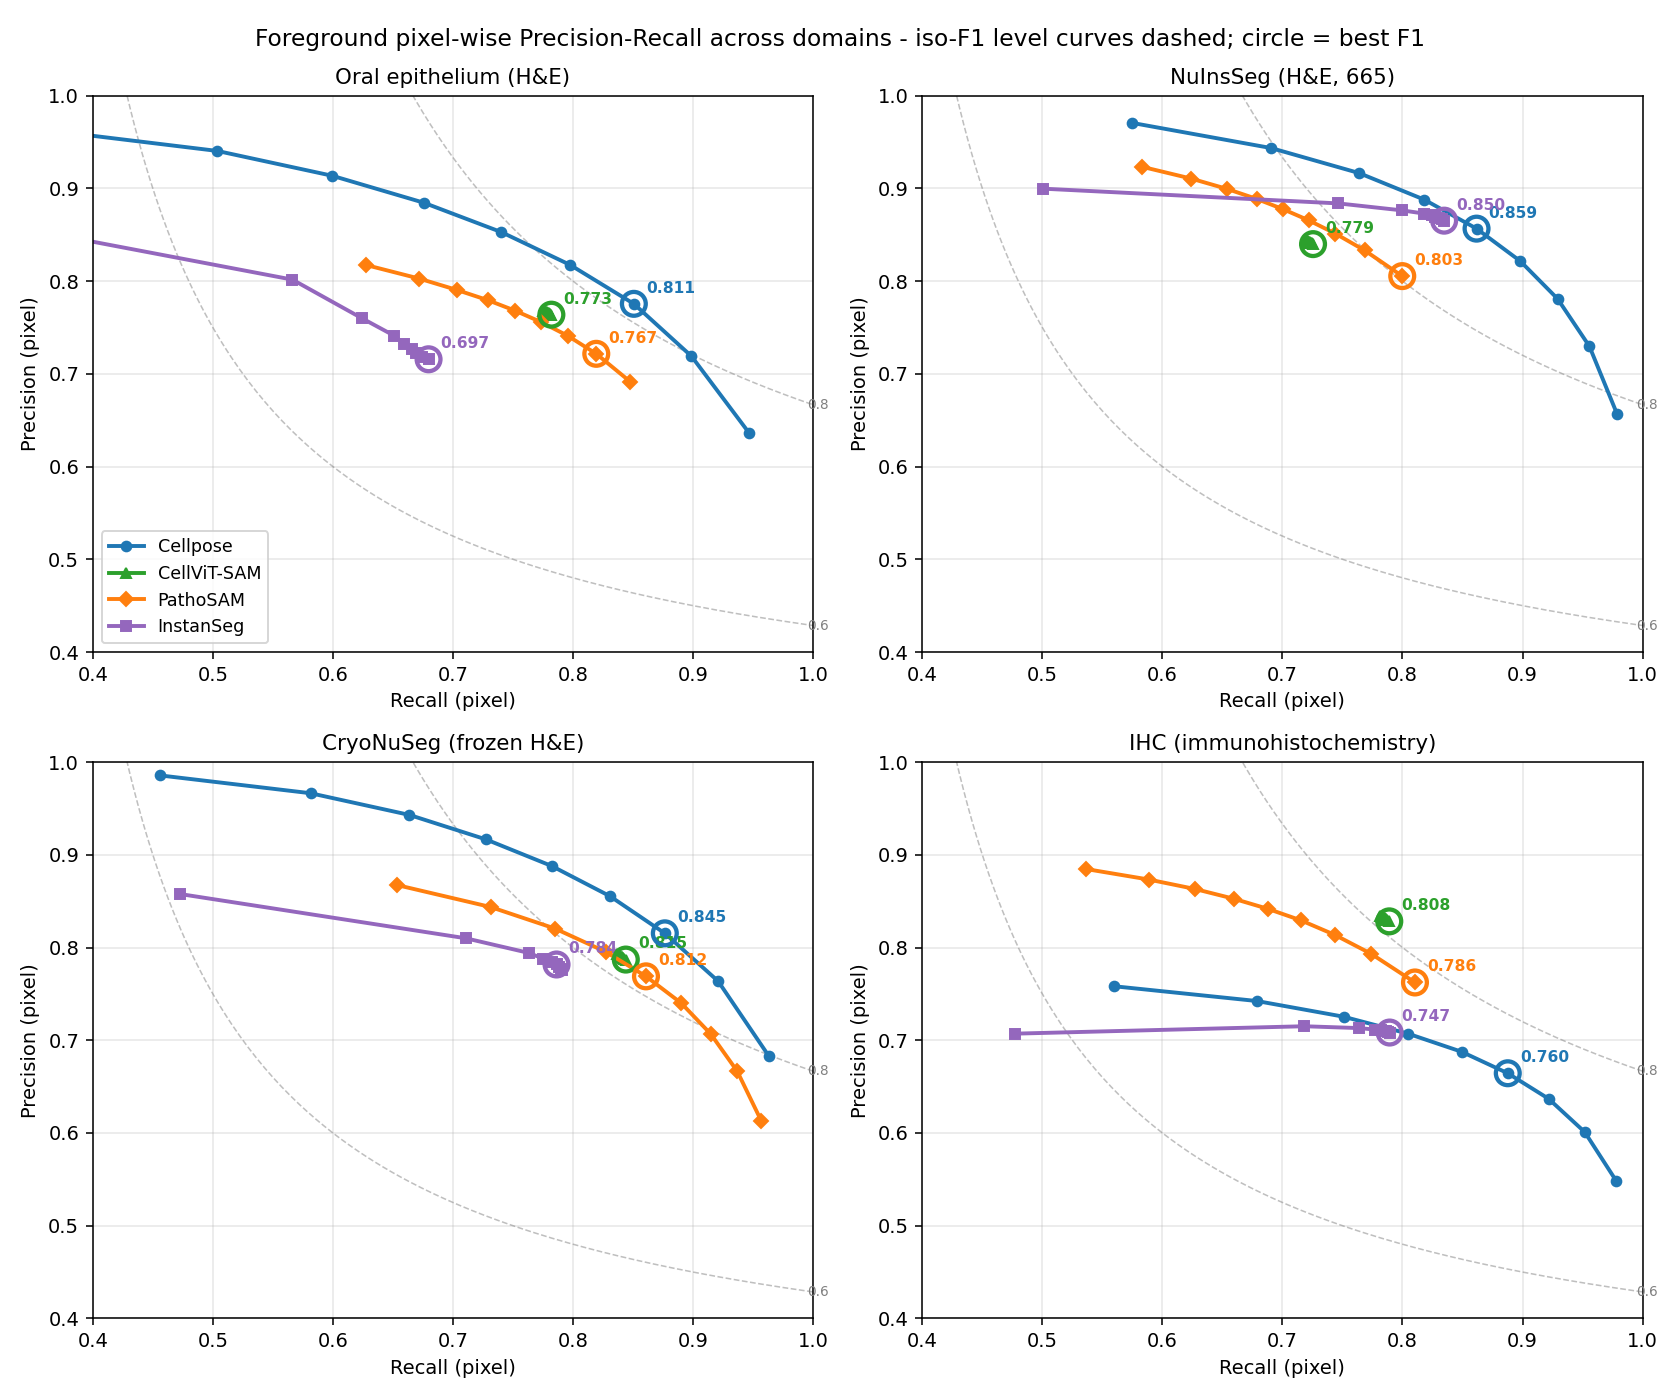
\includegraphics[width=\textwidth]{pr_pixel_crossdomain.png}
\caption{Foreground pixel-wise precision--recall across the four datasets in a single
view. Dashed lines are iso-F1 level curves; the open circle marks each model's
best-F1 operating point; points along a curve are detection thresholds
$p\in\{0.1,\dots,0.9\}$. The ranking \emph{inverts} with the staining: Cellpose
leads on the three H\&E sets (oral, NuInsSeg, CryoNuSeg) while CellViT leads on IHC.
Cellpose is shown without its flow-error filter.}
\label{fig:crossdomain}
\end{figure*}

\subsection{The ranking depends on the metric}
The chosen metric also shifts the comparison (Table~\ref{tab:combined}, Fig.~\ref{fig:boundarycd}). Under the
boundary analysis, the models achieve \emph{comparable boundary recall} (they
recover similar fractions of the true nuclear contours), yet on the oral and
CryoNuSeg H\&E sets Cellpose attains the highest boundary-F because it produces
fewer spurious edges (higher boundary precision); on NuInsSeg, InstanSeg edges it
by $0.006$. Thus a recall-only reading would call the models close to a tie,
whereas the precision-weighted F-score favors Cellpose on the oral and cryosection
H\&E sets.
Notably, the boundary-F ranking shows the same domain inversion as the pixel
metric: on IHC the best boundary-F belongs to CellViT, not Cellpose. The
background-inclusive variant pushes all models close to 1.0 because the
large amount of background pixels is easy to classify and dominates the score. Because of
this, we use the foreground-only metric as our main pixel metric and include the
background-inclusive one only as an ablation study.
Across all domains the boundary scores sit well below the pixel-overlap scores (best
boundary-F $0.52$--$0.76$ vs.\ pixel-F1 $0.76$--$0.86$), the quantitative signature that
the contour is recovered less reliably than the nuclear interior (Fig.~\ref{fig:boundarycd}).

\begin{figure*}[t]
\centering
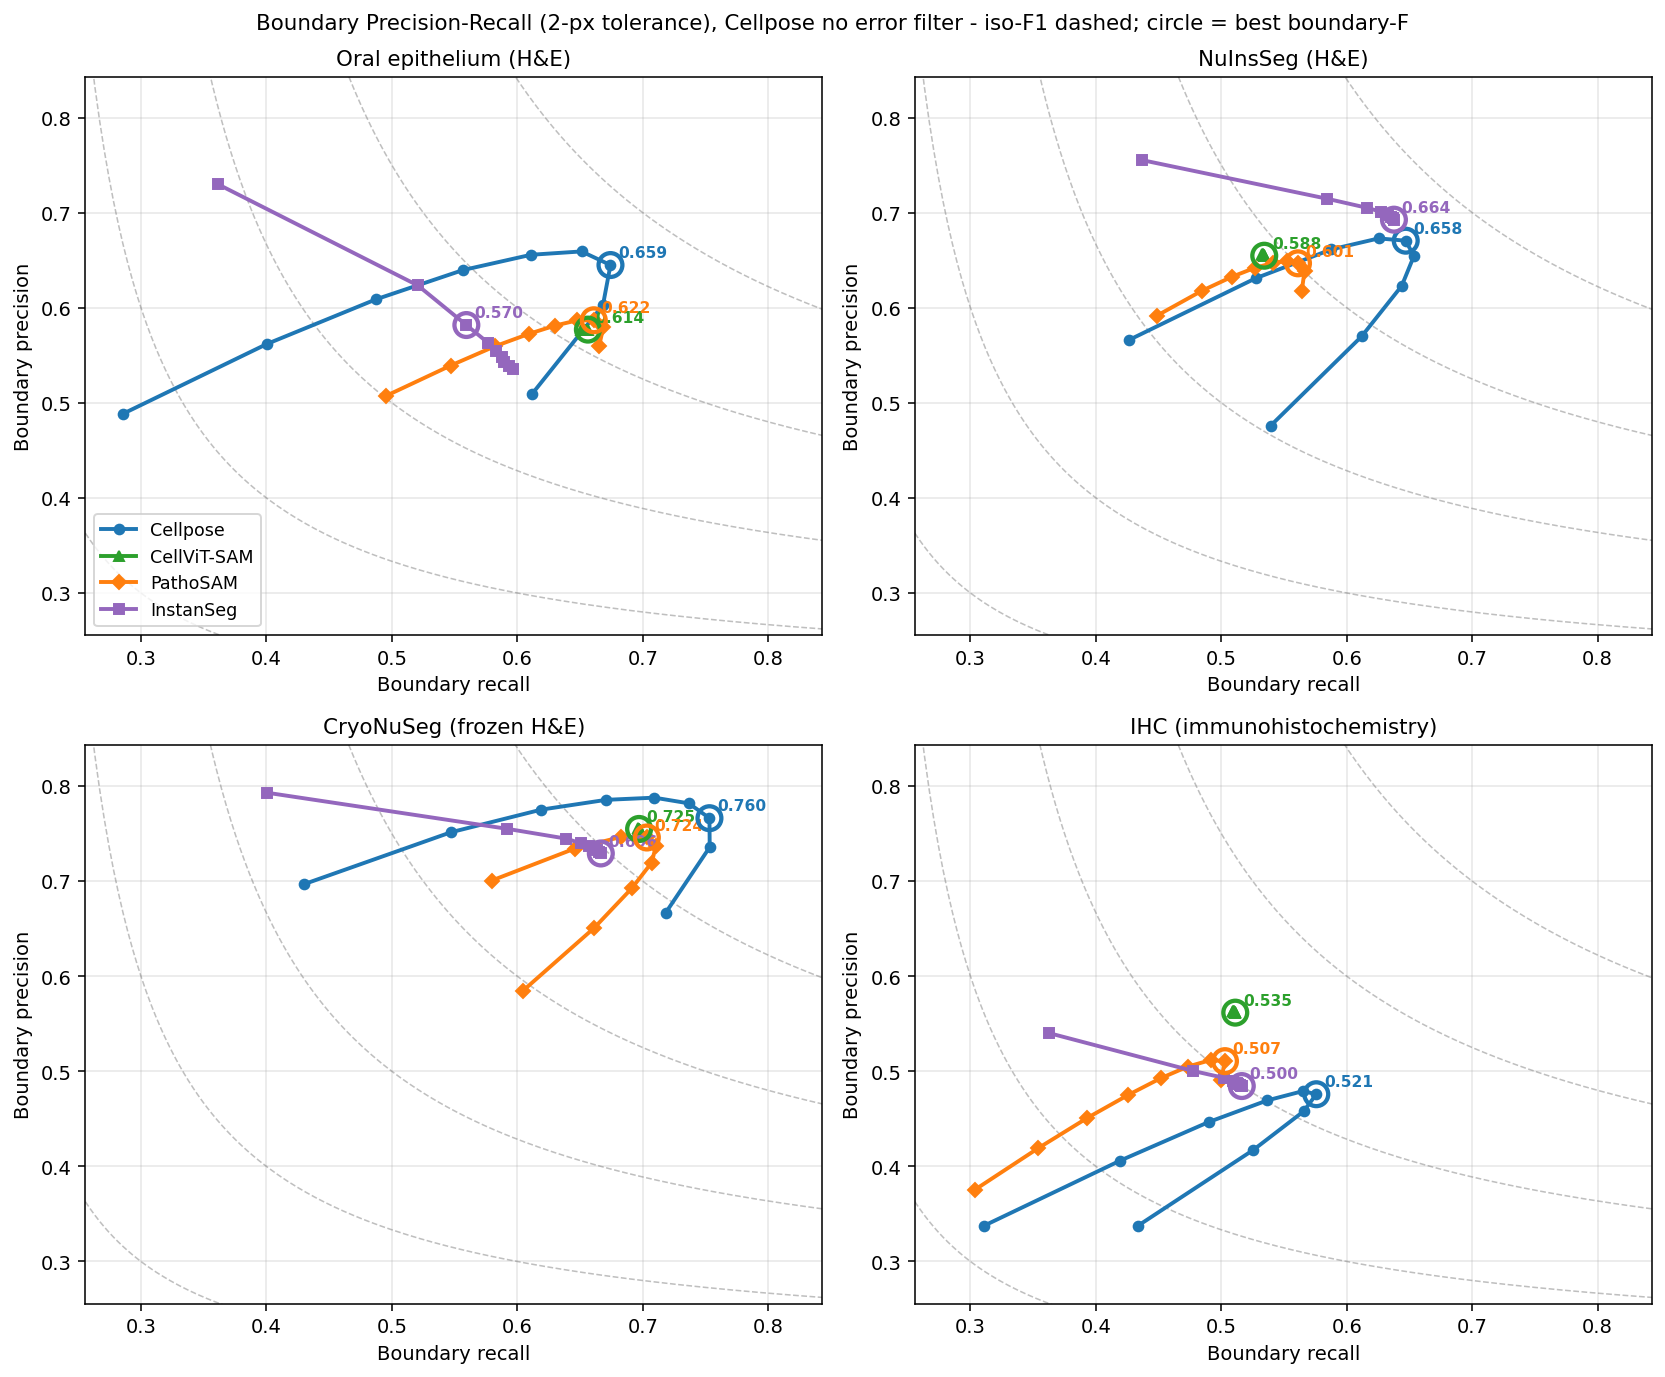
\includegraphics[width=\textwidth]{pr_boundary_crossdomain.png}
\caption{Boundary precision--recall (2-px tolerance) across the four datasets, Cellpose
without its flow-error filter. Iso-F1 level curves are dashed; the open circle marks each
model's best boundary-F. The boundary scores sit markedly lower than the pixel scores of
Fig.~\ref{fig:crossdomain}: recovering the exact contour is harder than covering the nucleus,
and it is where the residual error concentrates.}
\label{fig:boundarycd}
\end{figure*}

\subsection{Why CellViT cannot be thresholded (saturation)}
The CellViT foreground probability is near-binary, so sweeping its threshold
barely changes the prediction (Fig.~\ref{fig:saturation}). This follows from its
Dice-style training loss, known to produce overconfident outputs~\cite{yeung2022}.

\begin{figure}[t]
\centering
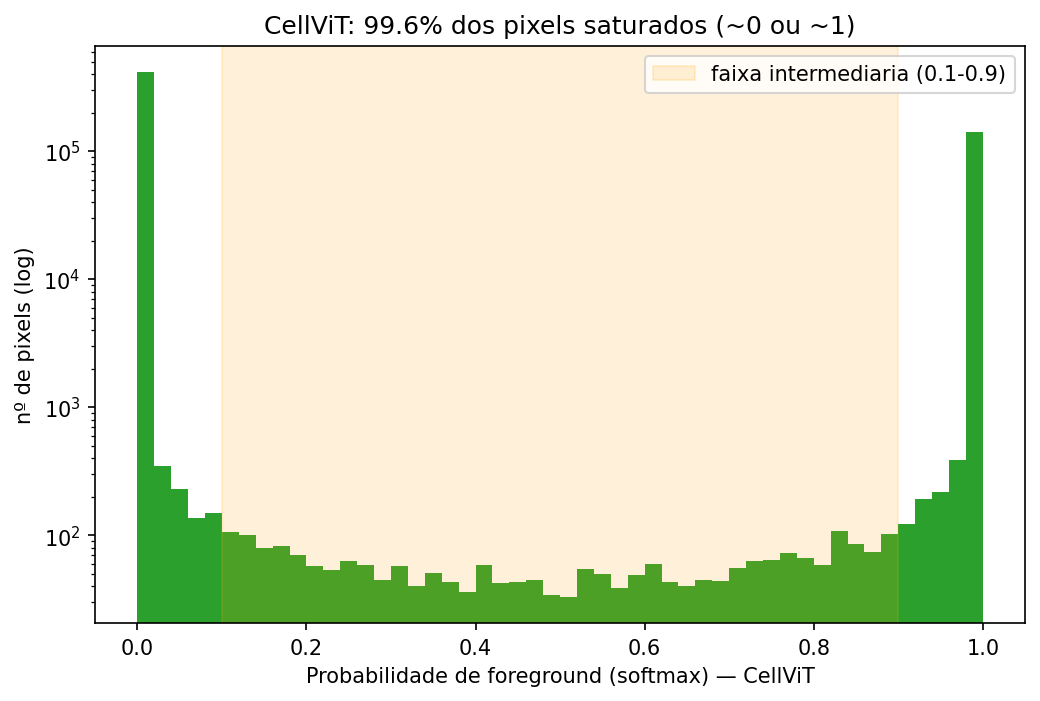
\includegraphics[width=0.85\linewidth]{cellvit_prob_histogram.png}
\caption{CellViT foreground-probability histogram: $\sim$99.6\% of pixels fall at
0 or 1, leaving almost nothing in the 0.1--0.9 band, so the detection threshold is inert.}
\label{fig:saturation}
\end{figure}

\subsection{Apparent superiority is a protocol effect, not delineation}

\begin{figure}[!t]
\centering
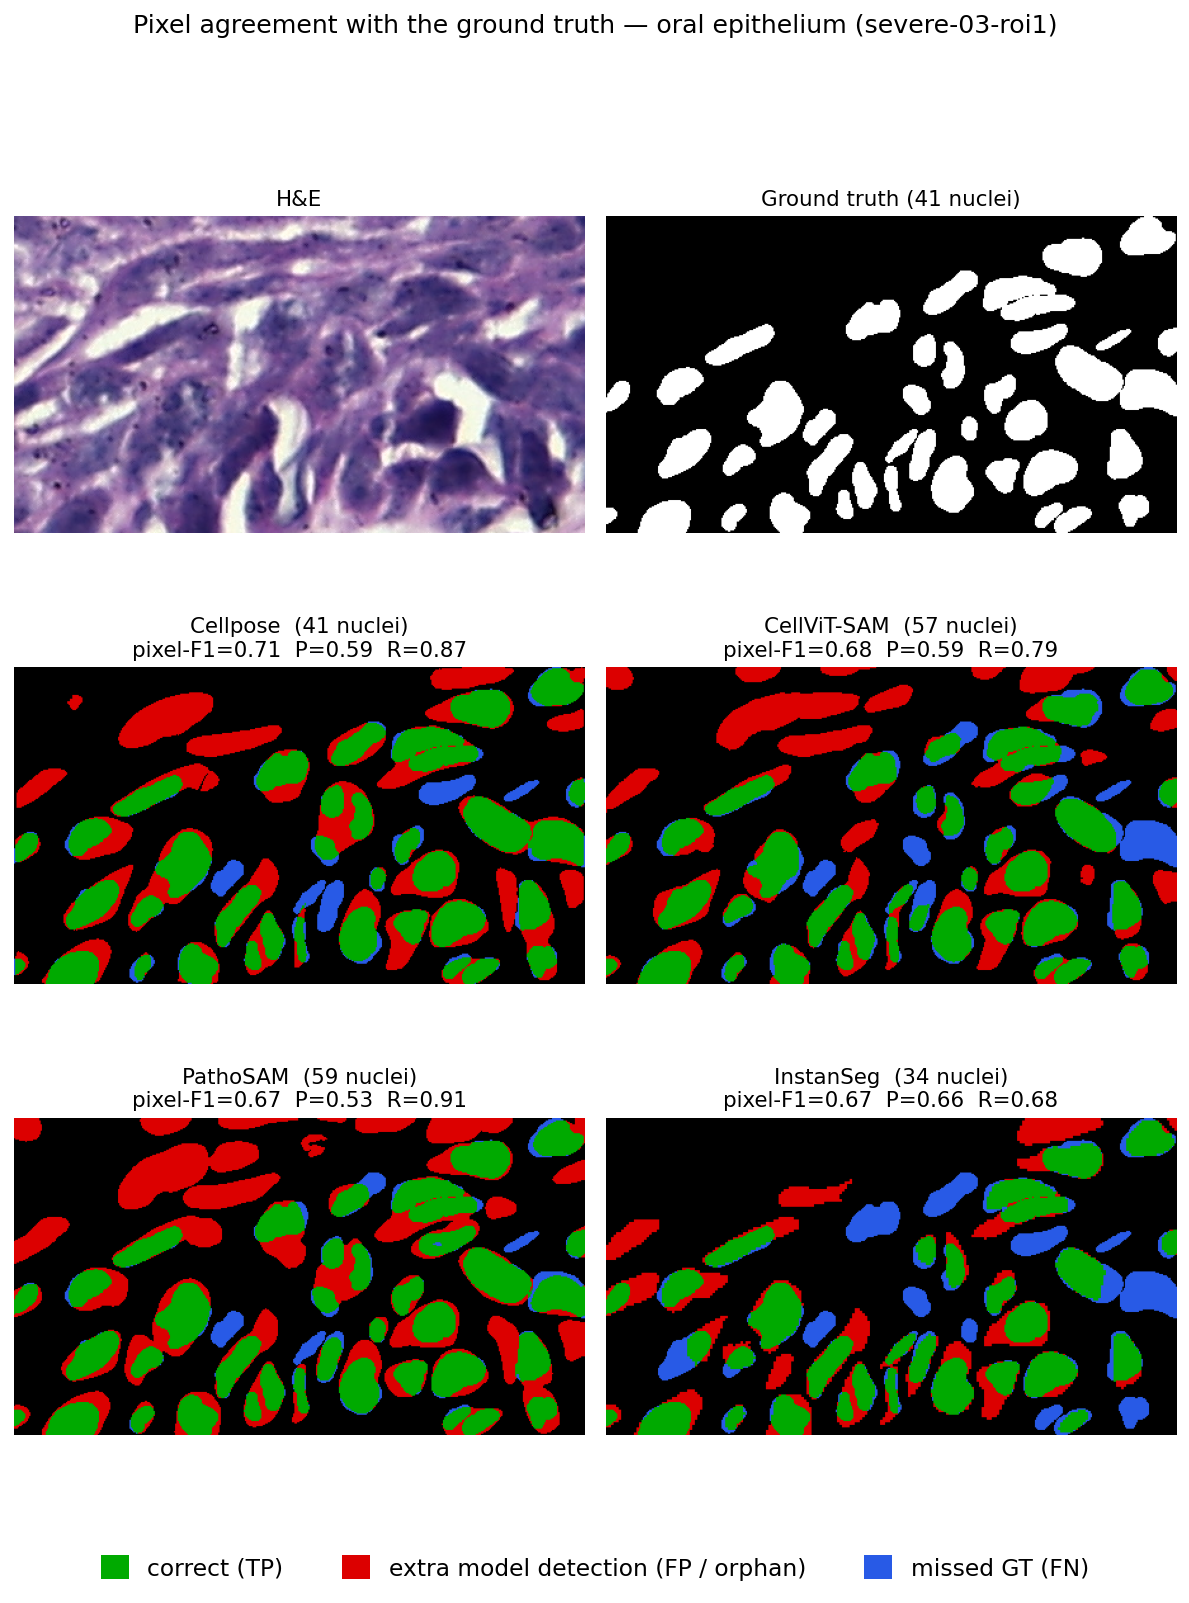
\includegraphics[width=\linewidth]{overlay_oral_protocol.png}
\caption{Pixel agreement with the ground truth on one oral ROI (\texttt{severe-03-roi1});
see the legend for the TP/FP/FN colors. The GT labels $41$ nuclei; Cellpose reports $41$ at
high precision ($P{=}0.71$), while the over-detecting models report many more ($57$ for CellViT,
$59$ for PathoSAM) and accumulate red (FP). The extra detections fall on real but un-annotated
nuclei, which the protocol counts as false positives, so the gap is in detection count, not in
how the matched nuclei are delineated. InstanSeg behaves in the opposite way here,
under-detecting ($34$ nuclei, more blue), consistent with it being the weakest model on the
oral set.}
\label{fig:protocol}
\end{figure}

A natural reading of the pixel-F1 gap is that Cellpose draws better masks than CellViT and
PathoSAM. The matched-nucleus numbers say otherwise: when a prediction is paired
with a ground-truth nucleus, all four models reach a very similar mean IoU
($\approx$0.74--0.76) and mean Dice ($\approx$0.85--0.86). In other words, once a nucleus is
found, every model traces roughly the same contour. The ranking is therefore not decided by
delineation quality.

What separates the models is \emph{how many} objects they report (Fig.~\ref{fig:protocol}).
CellViT and PathoSAM are generic nucleus finders and consistently detect
more candidates than Cellpose. We inspected where their non-matched predictions fall: for
Cellpose, $78\%$ of predictions match a GT nucleus and only $15\%$ are unmatched false positives
(masks on a region the GT leaves empty), whereas for CellViT and PathoSAM the matched fraction
drops to $53$--$55\%$ and the unmatched fraction rises to $27$--$28\%$. These extra detections are penalised as false
positives, which lowers precision and, with it, the precision-weighted pixel- and boundary-F
scores where Cellpose leads. Boundary recall tells the complementary story: these two detectors cover
a similar or larger fraction of the true contours precisely because they detect more nuclei
(Table~\ref{tab:combined}). The gap is thus a property of the detection count and the
evaluation protocol, not of contour accuracy.

We add one caveat. Whether these unmatched detections are genuine false positives or real nuclei
that the GT does not annotate is a question we cannot fully settle without a pathologist
re-reading the slides. On the oral set, the overlay in Fig.~\ref{fig:protocol} suggests the GT
annotates a specific subset of nuclei and skips others that CellViT and PathoSAM still detect, which
would make part of the unmatched count an annotation-coverage effect rather than a model error. We
treat this only as an observation and keep it out of our quantitative claims.

\subsection{Seeded interactive segmentation with NuClick}
\label{sec:seeded}

\begin{figure*}[!t]
\centering
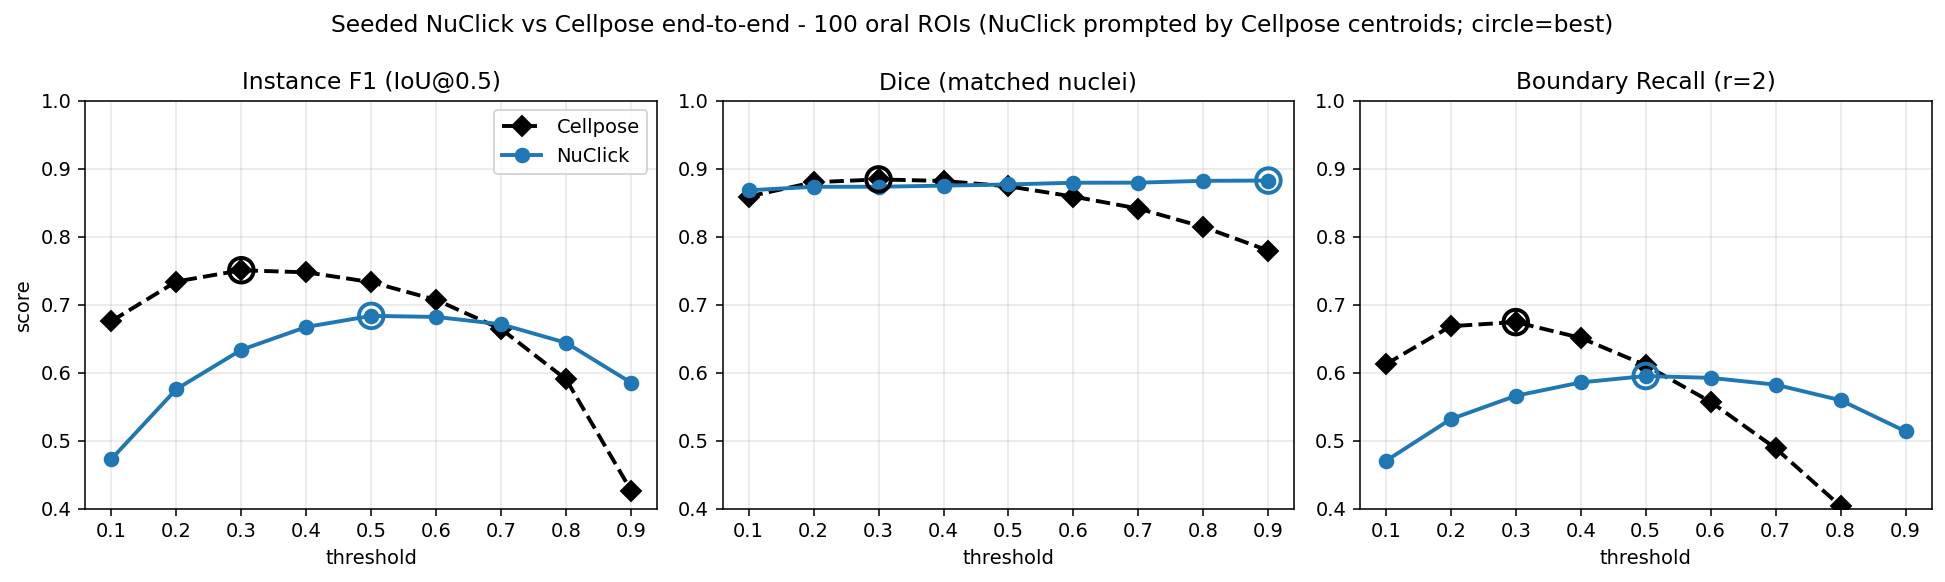
\includegraphics[width=\textwidth]{study_3metrics_full.png}
\caption{NuClick vs.\ Cellpose on 100 oral ROIs (F1 / Dice / boundary
recall vs.\ threshold). NuClick is an interactive segmenter here prompted with
\emph{automatic} Cellpose-probability centroids. On matched nuclei the delineation is
competitive: Dice is very close for Cellpose and NuClick ($\sim$0.87--0.88), and
NuClick recovers most of Cellpose's detections. Under automatic prompts, the seeded
pipeline does not beat the end-to-end model at its best operating point.}
\label{fig:seeded}
\end{figure*}

\textbf{A separate category.} Unlike the four standalone detectors above, NuClick does not localize
cells on its own: it is a \emph{seeded} segmenter that requires a probability map (or click prompts)
from an upstream detector as input. We therefore treat it as its own category, evaluating a
Cellpose$+$NuClick pipeline rather than ranking NuClick directly against the end-to-end models.
We want to know whether this pairing can reach the quality of an end-to-end model. We use the full
oral set (100 ROIs) and take the centroids
of Cellpose's probability map (thresholded at $p$) as automatic click prompts. The centroids
feed the click-based segmenter NuClick~\cite{nuclick} (a click-guided CNN). NuClick is an
\emph{interactive} method designed for human-placed clicks; here it receives automatic centroids,
so its scores lower-bound its interactive performance. This is therefore a feasibility probe of an
automatic seed-and-segment pipeline, not a head-to-head ranking. Because Cellpose and NuClick share
the same detections, the comparison isolates the segmentation step. We report instance F1, Dice on
matched nuclei, and boundary recall (Fig.~\ref{fig:seeded}, Table~\ref{tab:seeded}).

\begin{table}[t]
\centering
\caption{Seeded NuClick vs.\ Cellpose end-to-end (best over
threshold, 100 oral ROIs). NuClick uses Cellpose-centroid prompts.}
\label{tab:seeded}
\adjustbox{max width=\columnwidth}{%
\begin{tabular}{lccc}
\toprule
Method & F1 (inst.) & Dice (matched) & Boundary recall \\
\midrule
Cellpose (end-to-end) & \textbf{0.751} & \textbf{0.884} & \textbf{0.674} \\
NuClick (seeded)      & 0.684 & 0.883 & 0.595 \\
\bottomrule
\end{tabular}}
\end{table}

Under automatic prompting, the seeded pipeline does not surpass the model that generates the seeds:
NuClick on Cellpose centroids recovers about 91\% of Cellpose's instance F1 (0.684 vs.\ 0.751) and is
almost tied on Dice, trailing only on boundary recall. We stress that NuClick is used outside its
intended human-in-the-loop regime, so these numbers lower-bound what it would reach with expert
clicks; in this automatic setting the end-to-end model remains the stronger choice.

\textbf{Does this hold across domains?}
The oral comparison above uses probability-map centroids. We also ran the Cellpose$+$NuClick pipeline
on a 100-patch sample of each dataset (CryoNuSeg has only 30), now seeding NuClick at the centroid of
each \emph{Cellpose instance} so that it inherits exactly Cellpose's detections
(Fig.~\ref{fig:seededcd}). Under this seeding the pipeline is competitive with end-to-end Cellpose
across all four domains: a paired image-level bootstrap (10k resamples, each method at its best
threshold) finds \emph{no} significant difference on oral ($+0.005$, $p{=}0.45$) or IHC
($-0.007$, $p{=}0.11$), a small but significant Cellpose lead on NuInsSeg ($-0.035$, $p{<}0.001$),
and a small significant NuClick lead on CryoNuSeg ($+0.014$, $p{<}0.001$). The gap is
dataset-dependent, with no systematic disadvantage for the seeded method. The seeding choice
dominates: on oral, NuClick rises from $0.684$ (probability-map centroids, Table~\ref{tab:seeded})
to $0.755$ (instance centroids), erasing its apparent deficit. The bottleneck for the seeded
pipeline is thus \emph{detection} (which seeds it receives), not delineation.

\begin{figure*}[!t]
\centering
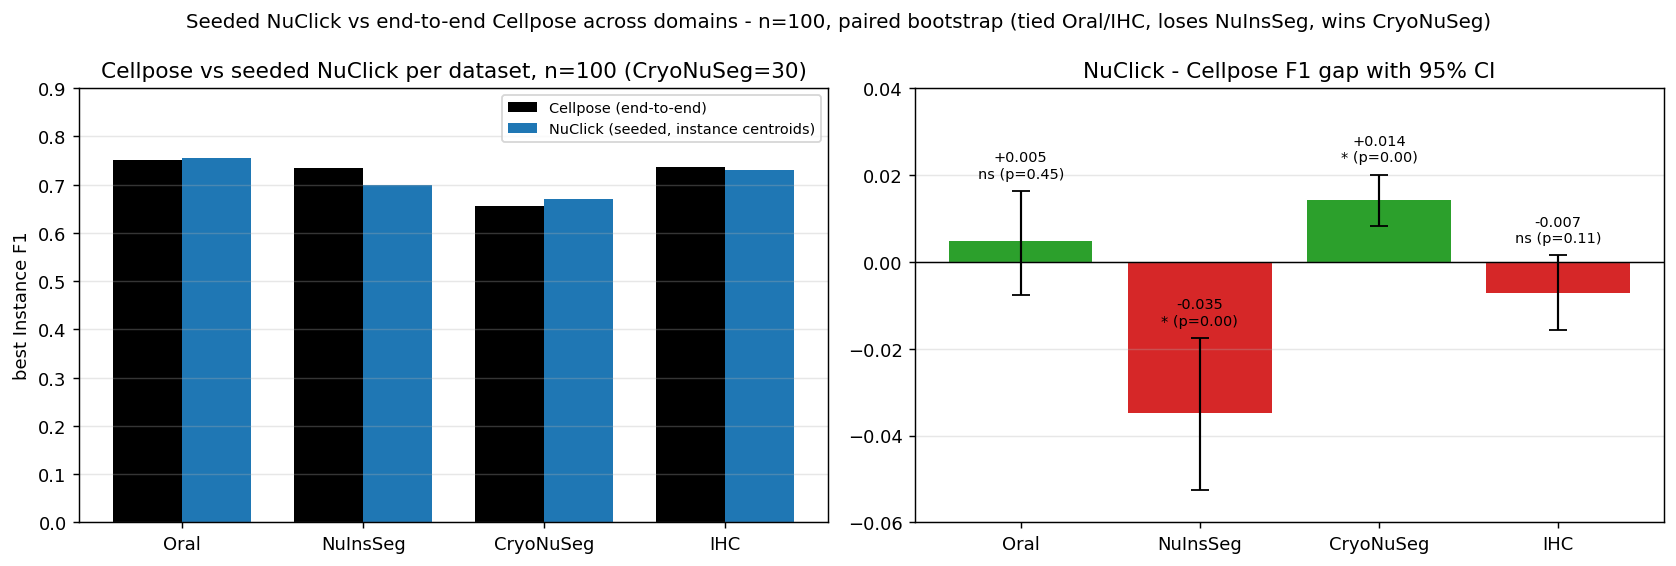
\includegraphics[width=\textwidth]{seeded_crossdomain.png}
\caption{Seeded NuClick vs.\ end-to-end Cellpose across four datasets ($n{=}100$; CryoNuSeg$=30$),
NuClick seeded at Cellpose-instance centroids. Right: NuClick$-$Cellpose best-F1 gap with 95\%
paired-bootstrap CI. NuClick is statistically tied on oral and IHC, loses on NuInsSeg, and wins on
CryoNuSeg. It is competitive across all four, with no systematic disadvantage for the seeded category.}
\label{fig:seededcd}
\end{figure*}

\textbf{Can we combine Cellpose and NuClick into something better?}
Since both methods give one mask per centroid, we can mix them with simple rules. We tried
two ideas and read both off the cached predictions, with no extra inference.

The first rule is \emph{max-area}: for each centroid, keep the larger of the two candidate
masks (the Cellpose instance or the NuClick mask). The best F1 is $0.704$ at $p{=}0.5$ and the
best Dice is $0.887$ at $p{=}0.3$. Picking the larger mask lifts Dice to essentially tie Cellpose,
but F1 stays below the end-to-end model: whenever NuClick's mask is the larger one it over-covers
the nucleus, and the extra pixels disagree with the GT, which hurts detection more than the slightly
tighter contour helps.

The second rule targets a specific failure mode we expected: Cellpose merging two touching nuclei
into one instance. The fix is to check, for every Cellpose instance, how many Cellpose centroids
fall inside it. If only one falls inside, we keep Cellpose. If two or more fall inside, we erase
the merged instance and repaint it with the NuClick mask of each centroid. The result is almost
identical to Cellpose alone (F1 $0.7494$ vs.\ $0.7506$ at $p{=}0.3$). The reason is interesting:
only \emph{8 splits out of 2362 Cellpose instances} (about $0.34\%$) actually trigger the rule at
$p{=}0.3$. In other words, Cellpose's flow tracking already separates touching nuclei well in this
dataset, even when the probability map shows the cells as a single connected blob. Under-merging is
not the bottleneck. The remaining gap is mostly detection of weak nuclei that Cellpose simply
does not pick up, which is a different problem that simple post-hoc rules cannot fix.

% =====================================================================
\section{Discussion}
\label{sec:discussion}
We can draw three main conclusions from our results. First, the best model depends on the dataset
type: Cellpose leads on the H\&E sets, but on IHC images, CellViT and PathoSAM
perform better. This split must be read together with training provenance
(Table~\ref{tab:traindata}): two of the three H\&E sets (NuInsSeg, CryoNuSeg) are in
Cellpose-SAM's training corpus, so its lead there cannot be attributed to generalization.
On the only fully held-out H\&E set (oral epithelium) Cellpose-SAM still leads, but this is a
single, narrow (murine) domain. The cross-domain inversion itself is robust to this caveat:
even where Cellpose-SAM trained on the data it does not win every metric (InstanSeg takes
boundary-F on NuInsSeg), and it loses outright on IHC, a dataset whose cohort it likely also
saw. This means that a model that ranks high on one stain type might not perform
as well on another, even on its own training distribution. Second, the best model depends on the metric used: pixel-wise foreground
scores favor Cellpose because it produces conservative, high-precision masks. On the other hand,
detection and boundary metrics favor CellViT and PathoSAM, which detect more nuclei but also produce
more false positives. Visual inspection shows that this difference is caused by how many nuclei are
detected, rather than the quality of the boundary contour, which is similar across models but
uniformly imperfect at the nuclear rim (boundary-F well below Dice); accurate boundary recovery is
thus a problem \emph{common} to all models rather than a differentiator between them. Third, the resulting ranking differs
from standard leaderboards: a model's apparent advantage on familiar data does not transfer
automatically to other domains.

A fourth observation comes from the seeded experiments in
Section~\ref{sec:seeded}: a click-based segmenter (NuClick) prompted with Cellpose centroids does
not beat Cellpose itself, and two simple ways of combining Cellpose and NuClick (max-area and
split-merged-instances) also fail to improve on the end-to-end model. The split-merged result is
the most informative one: only a tiny fraction of Cellpose instances ($\sim$0.3\% at $p{=}0.3$)
contain more than one probability-map centroid, which means Cellpose is not silently merging
touching nuclei in this dataset; its flow tracking handles them well. The remaining gap is in
detecting weak nuclei that Cellpose misses, which a downstream segmenter cannot recover.

\textbf{Limitations.} \emph{Training-set overlap.} The two generalist models
(Cellpose-SAM, InstanSeg) were trained on public corpora that include NuInsSeg,
CryoNuSeg and/or an IHC-TMA set, whereas the two transformer models (CellViT,
PathoSAM) were not; only the oral set is held-out for all four
(Table~\ref{tab:traindata}). We disclose this per model and avoid claiming
generalization on the affected sets, but it means the H\&E comparison is not a
clean cross-domain test for every model. Beyond this, our test datasets are
relatively small, so we calculate combined metrics
and leave statistical significance testing for future work. Also, we did not have a pathologist
check model detections that had no matching ground truth. Because of this, we cannot tell if these
are actual false positives or just nuclei that were missed in the manual annotations. Finally, the
IHC stain is far from the H\&E images that dominate every model's training, so the IHC results
should be seen as a robustness test rather than a standard comparison, noting that Cellpose-SAM
and InstanSeg may have seen an IHC-TMA set from the same cohort (Table~\ref{tab:traindata}), which
makes CellViT's lead there, as a model that did not, more striking.

% =====================================================================
\section{Conclusion}
\label{sec:conclusion}
We evaluated four pre-trained nucleus segmentation models on four unseen datasets (H\&E and IHC),
with pixel-wise, boundary, and threshold-sweep metrics. Three messages emerge.
First, there is \emph{no universal winner}: the best model depends on the dataset and the metric,
and an apparent advantage is often an artifact of the evaluation protocol (driven by how many
objects a model detects) rather than by contour quality.
Second, once a nucleus is matched, all four models trace nearly the same contour and reach the same
pixel overlap (Dice $\sim$0.85), and even a seeded segmenter (NuClick) does not improve on it. This does \emph{not} mean delineation is solved: pixel-overlap metrics are dominated
by the trivial nuclear interior and hide that the \emph{boundary} (where the residual error
geometrically concentrates) is recovered far less well (boundary-F of $0.5$--$0.76$ vs.\ Dice
$\sim$0.85). Because downstream morphometry reads the chromatin-density distribution \emph{inside}
the segmented mask~\cite{shifaterabbi2025}, an inaccurate boundary perturbs exactly the signal that
separates benign from malignant nuclei, and a smoothed contour also hides the membrane irregularity
used for grading; the contour, not the interior, is the part that still needs work.
Third, the remaining gap to the reference is \emph{detection}: the weak, low-contrast nuclei the
models miss entirely (Cellpose misses them rather than merging them; Sec.~\ref{sec:seeded}), which
post-hoc segmentation cannot recover.
We thus frame two open problems for the field: recovering the missed nuclei without inflating false
positives, and recovering the exact boundary that carries the morphometric signal. We recommend
choosing models with datasets and metrics matched to the application, and reporting boundary
fidelity alongside overlap. In future work we plan statistical testing on larger cohorts, more IHC
data, and detection-recovery targeted at the weak-nucleus bottleneck.

\bibliographystyle{IEEEtran}
\bibliography{refs}

\end{document}
